\documentclass{article}
\usepackage[utf8]{inputenc}
\usepackage{amsmath}
\usepackage[spanish]{babel}
\usepackage{graphicx}
\usepackage{float}
\newcommand\tab[1][1cm]{\hspace*{#1}}
\begin{document}



\section*{Tarea 3}
Nombre: Juan Sebastian Vargas\\
Fecha: 4/05/16

\subsection*{Punto 1}
\subsubsection*{Floyd-Warshall}
Para Solucionar este problema se utilizaria el mismo algoritmodescrito en \ref{FW}, donde $D^*$ es la matriz que contiene el costo minimo de los viajes. 

\begin{figure}[H]
\begin{center}
 \scalebox{0.5}{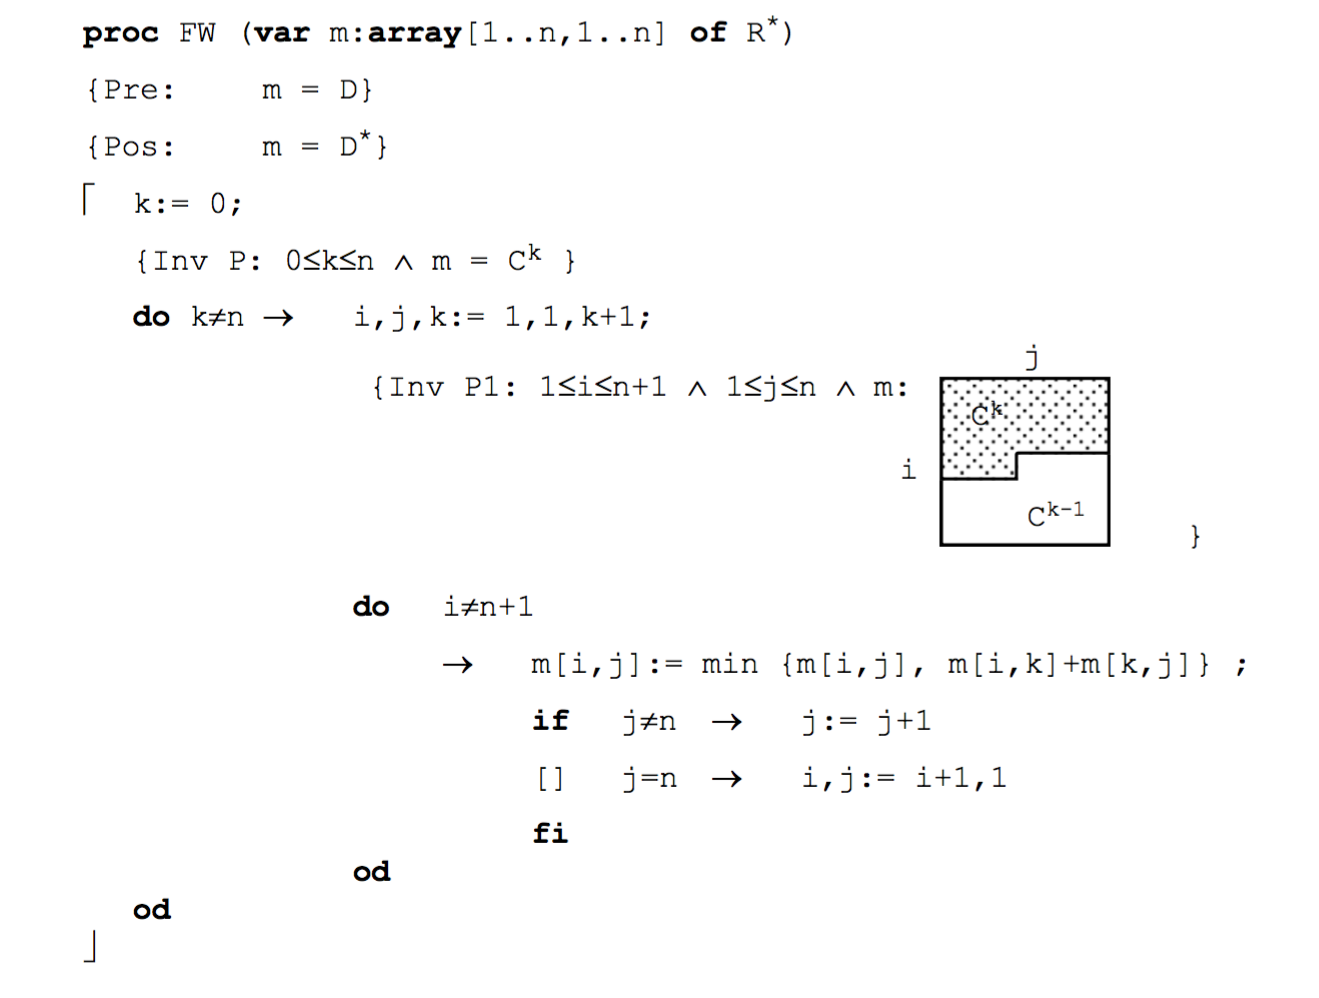
\includegraphics{FW.png}} 
 \caption{Floyd-Warshall ejemplo libro}
 \label{FW}
 \end{center}
\end{figure}
si se necesitara encontrar y reconstruir ese camino, se haria el mismo algoritmo, solo que actualizando una matriz tal que:

\begin{figure}[H]
\begin{center}
 \scalebox{0.5}{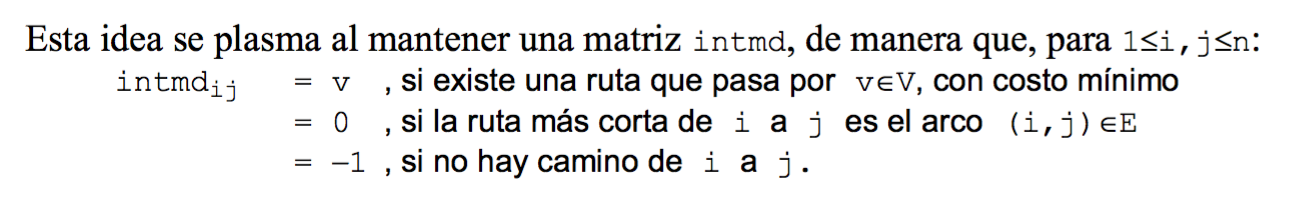
\includegraphics{intmd.png}} 
 \caption{Matriz para reconstruir el camino de costo minimo}
 \label{intmd}
 \end{center}
\end{figure}
 
 Para la complejidad temporal podemos encontrarla facilmente, como vemos en el algoritmo variamos i, j y k hasta n, donde n es el numero total de Nodos, y $T_{FW}=O(n^3)$, para la comlejidad Espacial tenemos guardamos una matriz de $nxn$ y es por esto que $S_{FW}=O(n^2)$

\subsubsection*{Dijkstra}
el algoritmo que me encuentra la ruta optima de un nodo f hasta el resto de nodos es: 

\begin{figure}[H]
\begin{center}
 \scalebox{0.5}{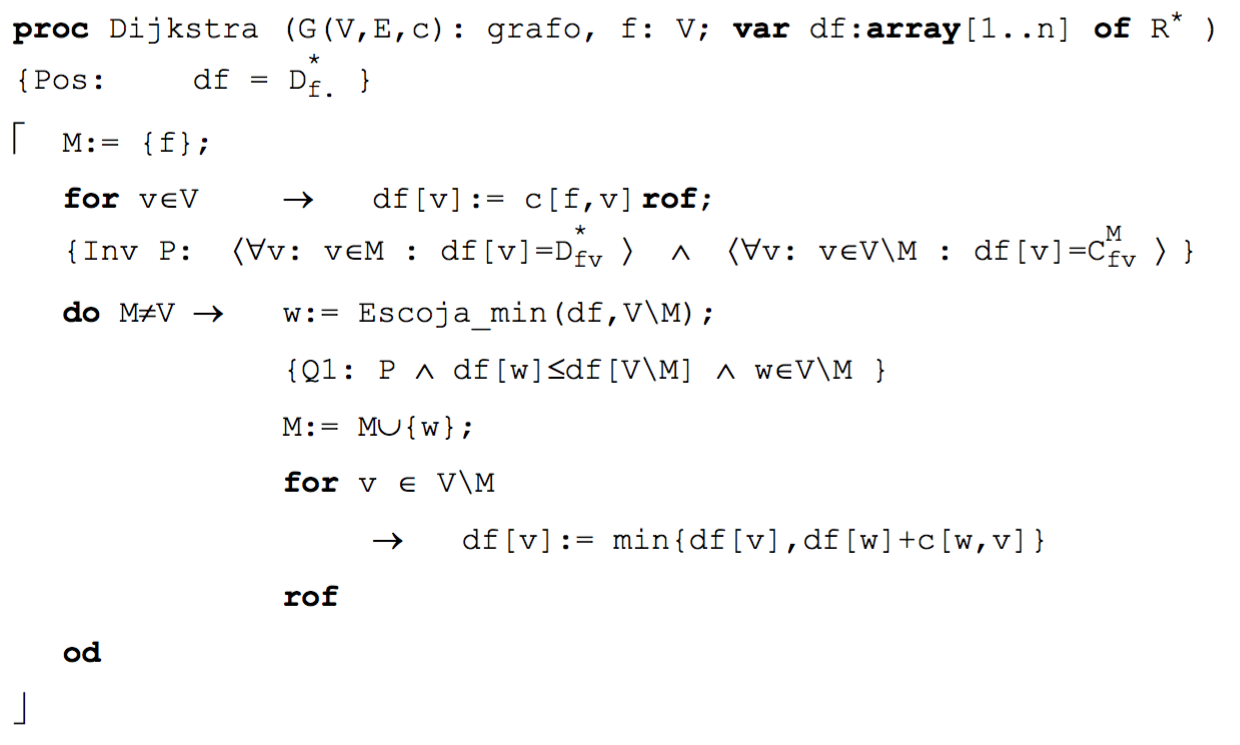
\includegraphics{dijkstra.png}} 
 \caption{Algoritmo de Dijkstra}
 \label{dijkstra}
 \end{center}
\end{figure}

donde la complejidad temporal depende de dos partes, la inicializacion y las iteraciones, la inicializacion es el primer for que llena el df, y las iteraciones son los ciclos que siguen.
\begin{equation}
T_D=T(Ini)+T(ciclos)=O(n)+O(n)[T(Escoja_min)+T(eliminar)]+O(e)
\end{equation}
Donde $T(Escoja_min)=O(n)$, ya que existen n diferentes nodos, teniendo todo en cuenta se obtiene que
\begin{equation}
T_D=O(n)[O(n)]+O(e)=O(n^2+e)
\end{equation}
pero esta seria la complejidad temporal para encontrar el camino minimo de un nodo dado f a el resto de los nodos del grafo, para obtener la totalidad de caminos minimos de todos los nodos hacia todos los nodos, debemos hacer este proceso para todos los nodos, en este casi la complejidad seria entonces:
\begin{equation}
T_{TD}=O(n(n^2+e))=O(n^3)
\end{equation}
donde se asumio que $e\ll n^3$, y para la espacial se guardara n vectores de la manera $di:i\in{1..f..n}$, y de esta manera $S_D=O(n^2)$


\subsection*{Punto 2}

\subsubsection*{2.a}
Para modelar este problema de esta manera tenemos un grafo $G(V,E,c)$debemos y definir cuando se llega a un estado de solucion, y esto pasa cuando:
\begin{equation}
v\in V: P=\sum_{i=1}^{n} c^v_i
\end{equation}
donde: 
\begin{equation}
c^v_i= \left\{ \begin{array}{lcc}
             c_i &   si  & v_i esta llena en v \\
             \\ 0 &  si & v_i esta vacia en v \\
              
             \end{array}
   \right.
\end{equation} 
\subsubsection*{2.b}



\subsection*{Punto 3}

\end{document}
